% !TeX encoding = UTF-8
% !TeX program = xelatex
% !TeX spellcheck = en_US

\documentclass[degree=doctor]{ustcthesis}
% degree      = doctor | master | bachelor
% degree-type = academic | professional
% language    = chinese | english
% fontset     = windows | mac | ubuntu | fandol

% 加载宏包、全部的配置
% !TeX root = ./main.tex

\ustcsetup{
  title              = {莫比乌斯带周围电场的计算和模拟},
  title*             = {Calculation and Simulation of Electric Field around Mobius Strip},
  author             = {李佩哲PB21051049~~~杨庆东PB21051052},
  author*            = {Li Peizhe, Yang Qingdong},
  speciality         = {910生命科学与医学部~~~209工程科学学院},
  speciality*        = {910~~Department of Life Sciences and Medicine\\~~~~~~~~~~~~~~~~~~~209~~College of Engineering Science},
  supervisor         = {卢荣德~教授, 孙霞~教授},
  supervisor*        = {Prof. Lu Rongde, Prof. Sun Xia},
  % date               = {2017-05-01},  % 默认为今日
  % professional-type  = {专业学位类型},
  % professional-type* = {Professional degree type},
  department         = {209工程科学学院~~~910生命科学与医学部},  % 院系,本科生需要填写
  student-id         = {PB21051049~PB21051052},  % 学号,本科生需要填写
  % secret-level       = {秘密},     % 绝密|机密|秘密|控阅,注释本行则公开
  % secret-level*      = {Secret},  % Top secret | Highly secret | Secret
  % secret-year        = {10},      % 保密/控阅期限
  %
  % 数学字体
  % math-style         = GB,  % 可选:GB, TeX, ISO
  math-font          = xits,  % 可选:stix, xits, libertinus
}


% 加载宏包

% 定理类环境宏包
\usepackage{amsthm}

% 插图
\usepackage{graphicx}

% 三线表
\usepackage{booktabs}

% 跨页表格
\usepackage{longtable}

% 算法
\usepackage[ruled,linesnumbered]{algorithm2e}

% SI 量和单位
\usepackage{siunitx}

% 参考文献使用 BibTeX + natbib 宏包
% 顺序编码制
\usepackage[sort]{natbib}
\bibliographystyle{ustcthesis-numerical}

% 著者-出版年制
% \usepackage{natbib}
% \bibliographystyle{ustcthesis-authoryear}

% 本科生参考文献的著录格式
% \usepackage[sort]{natbib}
% \bibliographystyle{ustcthesis-bachelor}

% 参考文献使用 BibLaTeX 宏包
% \usepackage[style=ustcthesis-numeric]{biblatex}
% \usepackage[bibstyle=ustcthesis-numeric,citestyle=ustcthesis-inline]{biblatex}
% \usepackage[style=ustcthesis-authoryear]{biblatex}
% \usepackage[style=ustcthesis-bachelor]{biblatex}
% 声明 BibLaTeX 的数据库
% \addbibresource{bib/ustc.bib}

% 配置图片的默认目录
\graphicspath{{figures/}}

% 数学命令
\makeatletter
\newcommand\dif{%  % 微分符号
  \mathop{}\!%
  \ifustc@math@style@TeX
    d%
  \else
    \mathrm{d}%
  \fi
}
\makeatother
\newcommand\eu{{\symup{e}}}
\newcommand\iu{{\symup{i}}}

% 用于写文档的命令
\DeclareRobustCommand\cs[1]{\texttt{\char`\\#1}}
\DeclareRobustCommand\pkg{\textsf}
\DeclareRobustCommand\file{\nolinkurl}

% hyperref 宏包在最后调用
\usepackage{hyperref}


\usepackage{listings}
\usepackage{fontspec} % 定制字体
\newfontfamily\menlo{Menlo}
\usepackage{xcolor} % 定制颜色
\definecolor{mygreen}{rgb}{0,0.6,0}
\definecolor{mygray}{rgb}{0.5,0.5,0.5}
\definecolor{mymauve}{rgb}{0.58,0,0.82}
\lstset{ %
backgroundcolor=\color{white},      % choose the background color
basicstyle=\footnotesize\ttfamily,  % size of fonts used for the code
columns=fullflexible,
tabsize=4,
breaklines=true,               % automatic line breaking only at whitespace
captionpos=b,                  % sets the caption-position to bottom
commentstyle=\color{mygreen},  % comment style
escapeinside={\%*}{*)},        % if you want to add LaTeX within your code
keywordstyle=\color{blue},     % keyword style
stringstyle=\color{mymauve}\ttfamily,  % string literal style
frame=single,
rulesepcolor=\color{red!20!green!20!blue!20},
% identifierstyle=\color{red},
language=c++,
}
\begin{document}

% 研究生论文:
%   封面,原创性声明和授权使用声明
%   frontmatter: 摘要,目录,[图、表清单],[符号说明]
%   mainmatter: 正文章节,参考文献
%   appendix: 附录
%   backmatter: 致谢,已发表论文列表
%
% 本科生论文:
%   封面
%   frontmatter: 致谢,目录,摘要
%   mainmatter: 正文章节,参考文献
%   appendix: 附录

\maketitle

\frontmatter
% !TeX root = ../main.tex

\ustcsetup{
  keywords = {
    物理化学实验, 表面张力
  },
  keywords* = {
    Physical chemistry experiment, Surface tension
  },
}

\begin{abstract}
  物体表面的分子和内部分子所处的境况不同,因而能量也不同,表面分子的能量比内部分子大.~
  表面张力。它表示表面自动缩小的趋势的大小.~
  表面张力是液体的重要特性之一,与所处的温度、压力、液体的组成共存的另一相的组成等有关.~
  纯液体的表面张力通常指该液体与饱和了其自身蒸气的空气共存的情况而言.~
  根据能量最低原理,溶质能降低溶液的表面张力时,表面层中溶质的浓度应比溶液内部大,反之,溶质使溶液的表面张力升高时,它在表面层中的浓度比在内部的浓度低.~
  这种表面浓度与溶液里面浓度不同的现象叫“吸附”.~
  表面活性物质具有显著的不对称结构,它是由亲水的极性部分和憎水的非极性部分构成.~
  正丁醇就是这样的分子,在水溶液表面的表面活性物质分子,其极性部分朝向溶液内部,而非极性部分朝向空气.~
  当表面张力仪中的毛细管截面与欲测液面相齐时,液面沿毛细管上升.~
  打开滴液漏斗的活塞,使水缓慢下滴而使体系内的压力增加,这时毛细管内的液面上受到一个比恒温试管中液面上稍大的压力,因此毛细管内的液面缓缓下降.~
  当此压力差在毛细管端面上产生的作用力稍大于毛细管口溶液的表面张力时,气泡就从毛细管口逸出.~
  这个最大的压力差可由数字式微压差测量仪上读出.~
  通过测定不同浓度正丁醇水溶液的表面张力,由曲线求溶液界面上的吸附量和单个正丁醇分子的横截面积.~
  了解表面张力的性质、表面能的意义以及表面张力和吸附的关系.~
  掌握一种测定表面张力的方法—最大气泡法.~
\end{abstract}

\begin{abstract*}
  Molecules on the surface of an object are in a different situation, and therefore have a different energy, than molecules in the interior, with surface molecules having more energy than interior molecules.
  Surface Tension. It indicates the magnitude of the tendency of a surface to shrink automatically.
  Surface tension is one of the most important properties of liquids and is related to the temperature, pressure, and composition of the other phase with which the liquid is coexisting.
  The surface tension of a pure liquid usually refers to the coexistence of the liquid with air saturated with its own vapor.
  According to the principle of energy minimization, when a solute lowers the surface tension of a solution, the concentration of the solute in the surface layer should be greater than in the interior of the solution, and conversely, when a solute raises the surface tension of a solution, its concentration in the surface layer is lower than in the interior.
  This difference between the concentration at the surface and the concentration inside the solution is called "adsorption".Adsorption
  Surface-active substances have a remarkable asymmetric structure consisting of a hydrophilic polar portion and a hydrophobic nonpolar portion.
  N-butanol is one such molecule, and the molecules of the surface-active substance on the surface of an aqueous solution have their polar portions oriented towards the interior of the solution and their non-polar portions oriented towards the air.
  When the cross section of the capillary in a surface tension meter is aligned with the surface of the liquid to be measured, the liquid surface rises along the capillary.
  The pressure in the system is increased by opening the piston of the dropping funnel and allowing the water to slowly drip down, the liquid level in the capillary tube is then subjected to a pressure slightly greater than that on the liquid level in the thermostat tube, and so the liquid level in the capillary tube slowly falls.
  When this pressure difference produces a force on the end face of the capillary that is slightly greater than the surface tension of the solution at the mouth of the capillary, bubbles escape from the capillary.
  This maximum pressure difference can be read on a digital differential pressure gauge.
  By measuring the surface tension of aqueous n-butanol solutions of different concentrations, the amount adsorbed at the solution interface and the cross-sectional area of a single n-butanol molecule are determined from the curves.
  Understand the nature of surface tension, the significance of surface energy, and the relationship between surface tension and adsorption.  Understand the significance of surface energy and the relationship between surface tension and adsorption.
  Knowledge of a method for determining surface tension, the maximum bubble method.  Understand the meaning of surface energy and the relationship between surface tension and adsorption.
\end{abstract*}

\tableofcontents
% \listoffigures
% \listoftables

\mainmatter
% !TeX root = ../main.tex

\chapter{绪论}
公元1858年,两名德国数学家莫比乌斯和Johann Benedict Listing分别发现,一个扭转180度后再两头粘接起来的纸条,具有魔术般的性质。
与普通纸带具有两个面(双侧曲面)不同,这样的纸带只有一个面(单侧曲面),一只小虫可以爬遍整个曲面而不必跨过它的边缘!
这一神奇的单面纸带被称为“莫比乌斯带”。作为一种典型的拓扑图形,莫比乌斯带引起了许多科学家的研究兴趣,并在生活和生产中有了一些应用。
例如,动力机械的皮带就可以做成“莫比乌斯带”状,这样皮带就不会只磨损一面了。
\cite{ref0}
实验室中也有可能产生莫比乌斯带形状的粒子。
一群科学家在Journal of Chemical Physics上发表了一篇论文,其中预言了一种莫比乌斯带形状的碳单质(准确来说应该是石墨烯)。
它能抵抗摄氏200度左右的温度,算是相当稳定。由于它莫比乌斯带的结构,它应该是一个偶极子,从而可以形成稳定的晶体。
\cite{ref00}

鉴于石墨烯可以带电,现假设某由石墨烯构成的莫比乌斯带均匀带电,以此来研究其周围空间中电场强度和电势的分布情况。
对于一个带电的物体,在计算它的电场时,可以把它分成若干小块,只要每个小块足够小,就可把每小块所带的电荷看成为点电荷,然后用点电荷电场叠加的方法计算整个带电体的电场。
\cite{ref01}
% !TeX root = ../main.tex

\chapter{浮动体}

\section{三线表}

三线表是《撰写手册》推荐使用的格式,如表~\ref{tab:exampletable}。
\begin{table}[h]
  \centering
  \caption{表号和表题在表的正上方}
  \label{tab:exampletable}
  \begin{tabular}{cl}
    \toprule
    类型   & 描述                                       \\
    \midrule
    挂线表 & 挂线表也称系统表、组织表,用于表现系统结构 \\
    无线表 & 无线表一般用于设备配置单、技术参数列表等   \\
    卡线表 & 卡线表有完全表,不完全表和三线表三种       \\
    \bottomrule
  \end{tabular}
  \note{注:表注分两种,第一种是对全表的注释,用不加阿拉伯数字排在表的下边,
    前面加“注:”;第二种是和表内的某处文字或数字相呼应的注,
    在表里面用带圈的阿拉伯数字在右上角标出,然后在表下面用同样的圈码注出来}
\end{table}

编制表格应简单明了,表达一致,明晰易懂,表文呼应、内容一致。
排版时表格字号略小,或变换字体,尽量不分页,尽量不跨节。
表格太大需要转页时,需要在续表上方注明“续表”,表头页应重复排出。



\section{插图}

有的同学可能听说“\LaTeX{} 只能使用 eps 格式的图片”,甚至把 jpg 格式转为 eps。
事实上,这种做法已经过时。
而且每次编译时都要要调用外部工具解析 eps,导致降低编译速度。
所以我们推荐矢量图直接使用 pdf 格式,位图使用 jpeg 或 png 格式。
\begin{figure}[h]
  \centering
  
\includegraphics[width=0.3\textwidth]{ustc-badge.pdf}
  \caption{图号、图题置于图的下方}
  \label{fig:badge}
  \note{注:图注的内容不宜放到图题中。}
\end{figure}

关于图片的并排,推荐使用较新的 \pkg{subcaption} 宏包,
不建议使用 \pkg{subfigure} 或 \pkg{subfig} 等宏包。



\section{算法环境}

模板中使用 \pkg{algorithm2e} 宏包实现算法环境。关于该宏包的具体用法,
请阅读宏包的官方文档。

\begin{algorithm}[h]
  \SetAlgoLined
  \KwData{this text}
  \KwResult{how to write algorithm with \LaTeX2e }

  initialization\;
  \While{not at end of this document}{
    read current\;
    \eIf{understand}{
      go to next section\;
      current section becomes this one\;
    }{
      go back to the beginning of current section\;
    }
  }
  \caption{算法示例1}
  \label{algo:algorithm1}
\end{algorithm}

注意,我们可以在论文中插入算法,但是插入大段的代码是愚蠢的。
然而这并不妨碍有的同学选择这么做,对于这些同学,建议用 \pkg{listings} 宏包。

% !TeX root = ../main.tex

\chapter{结果结论}
图\ref{EEE}和图\ref{UUU}分别显示了莫比乌斯岛周围的电场、电势分布状况。
\begin{figure}[h]
  \centering
  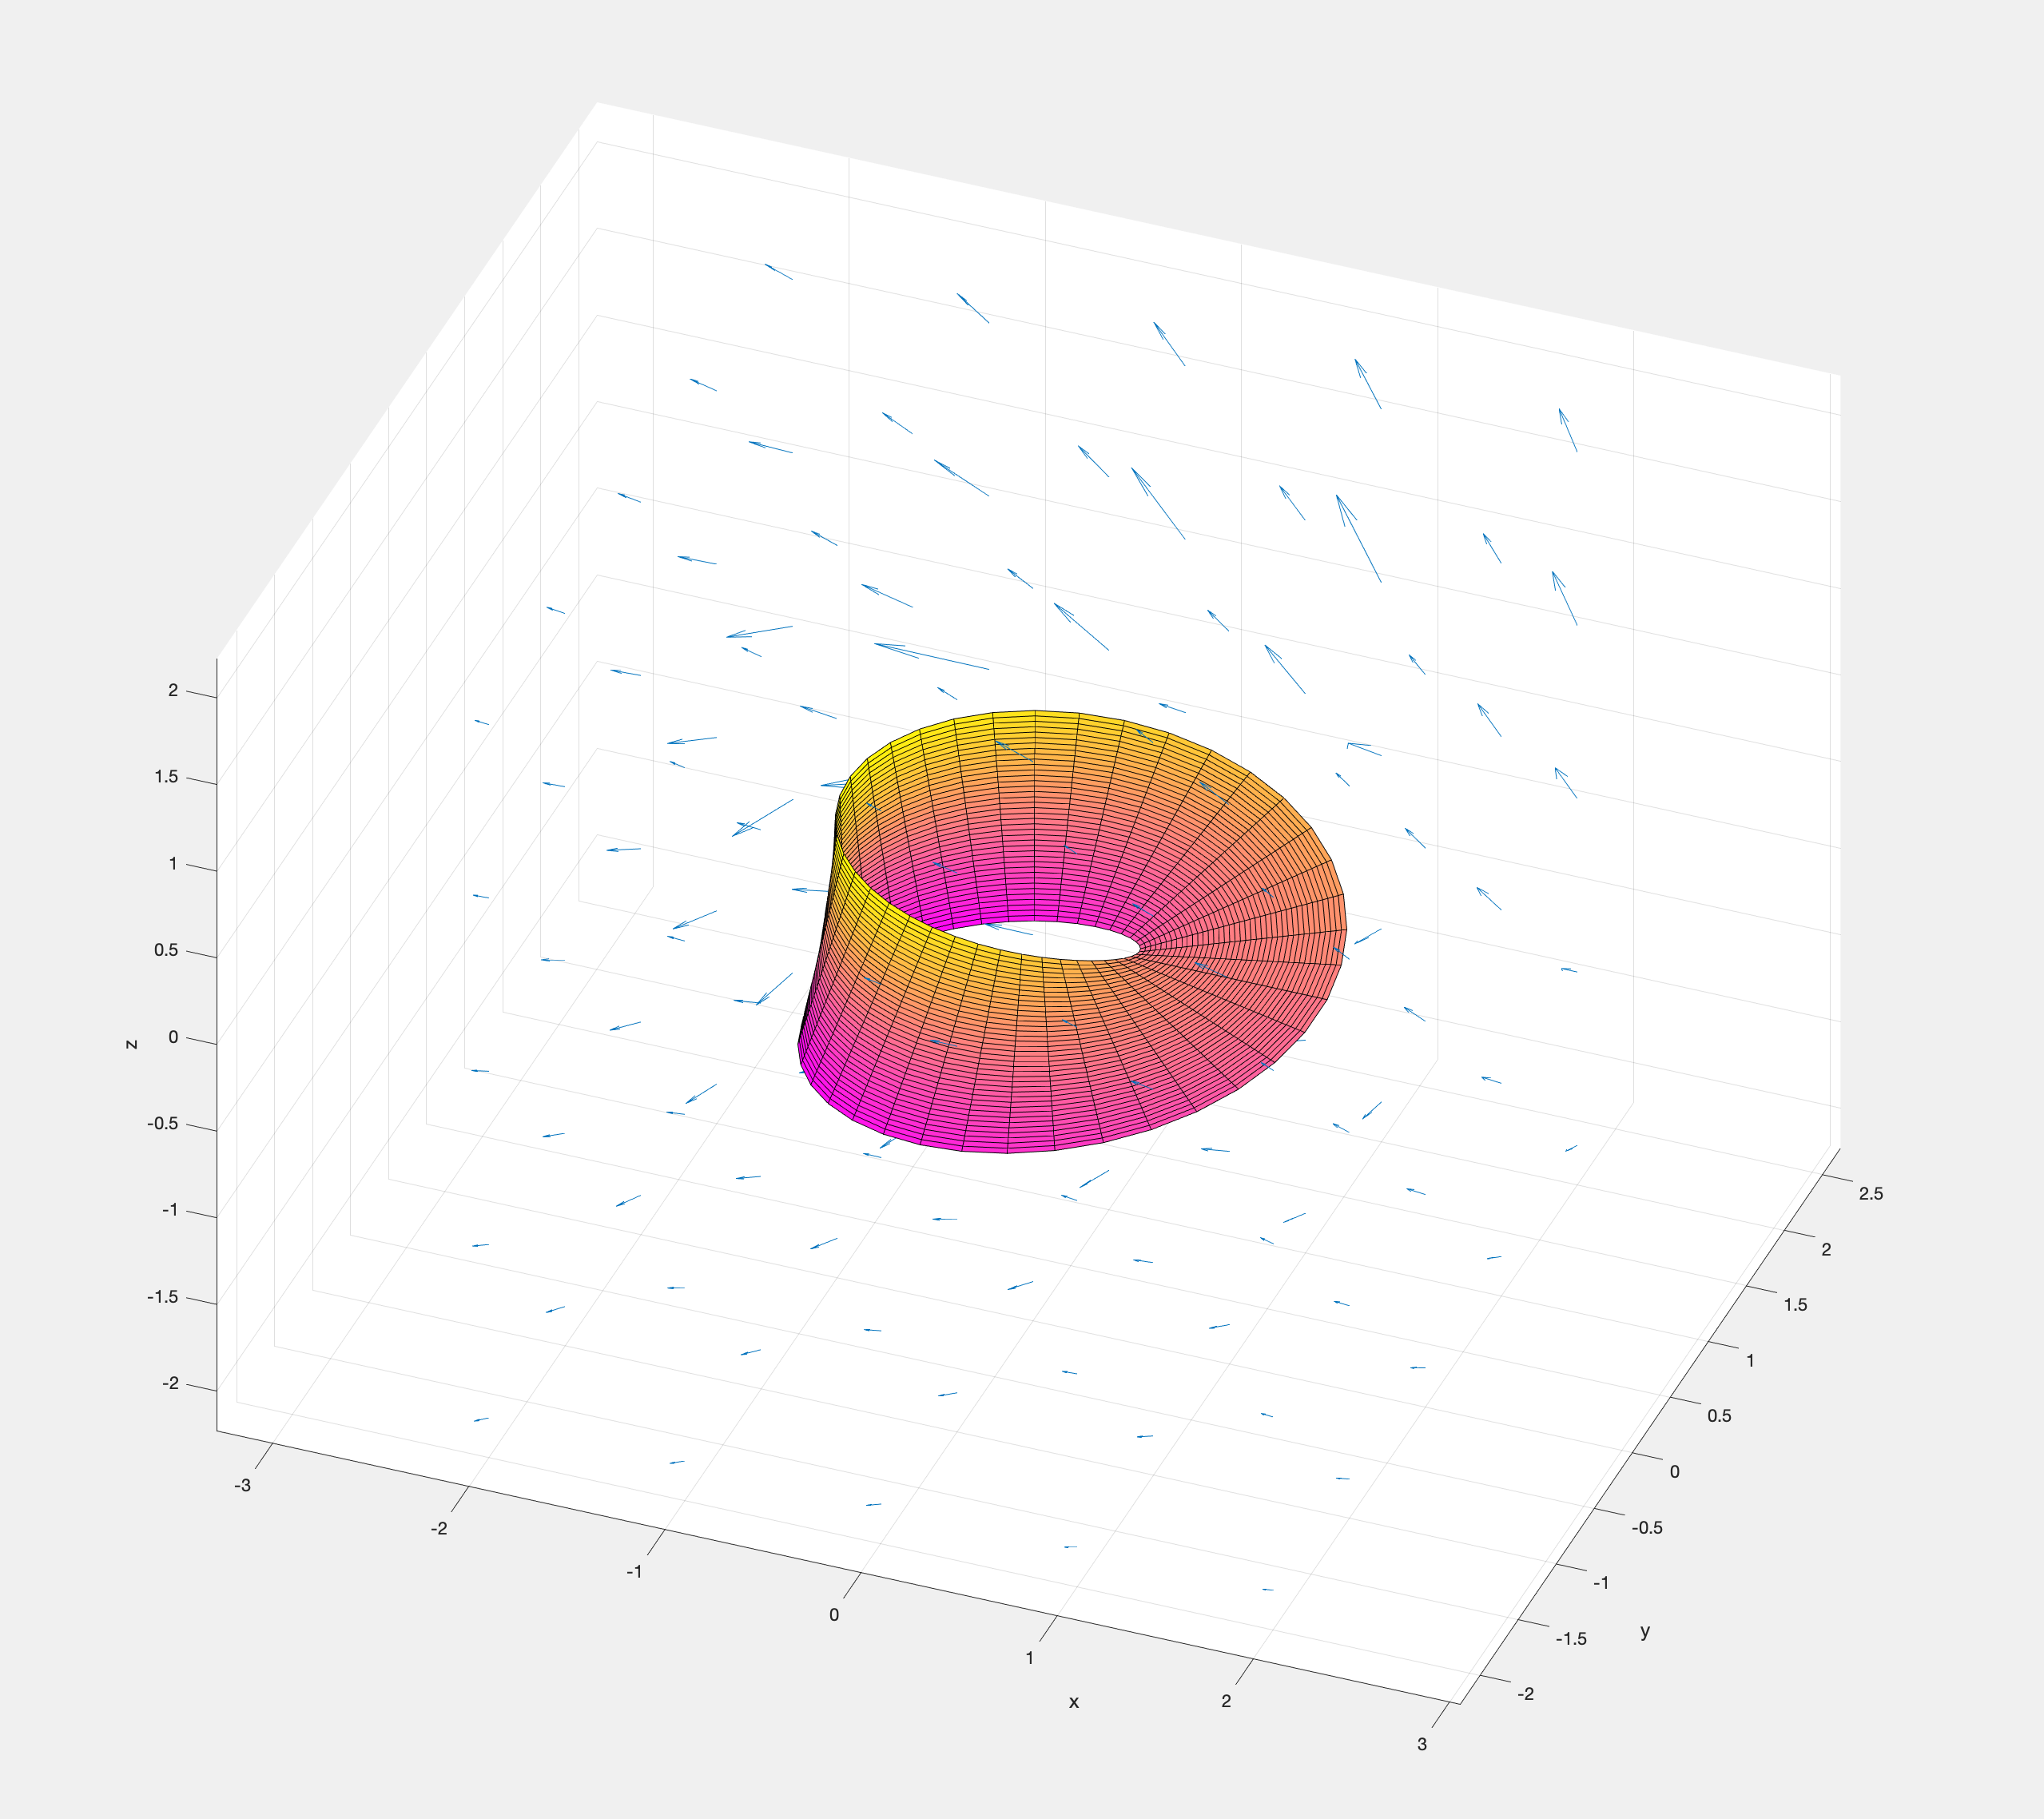
\includegraphics[width=0.7\textwidth]{E.png}
  \caption{莫比乌斯带周围电场的分布}\label{EEE}
  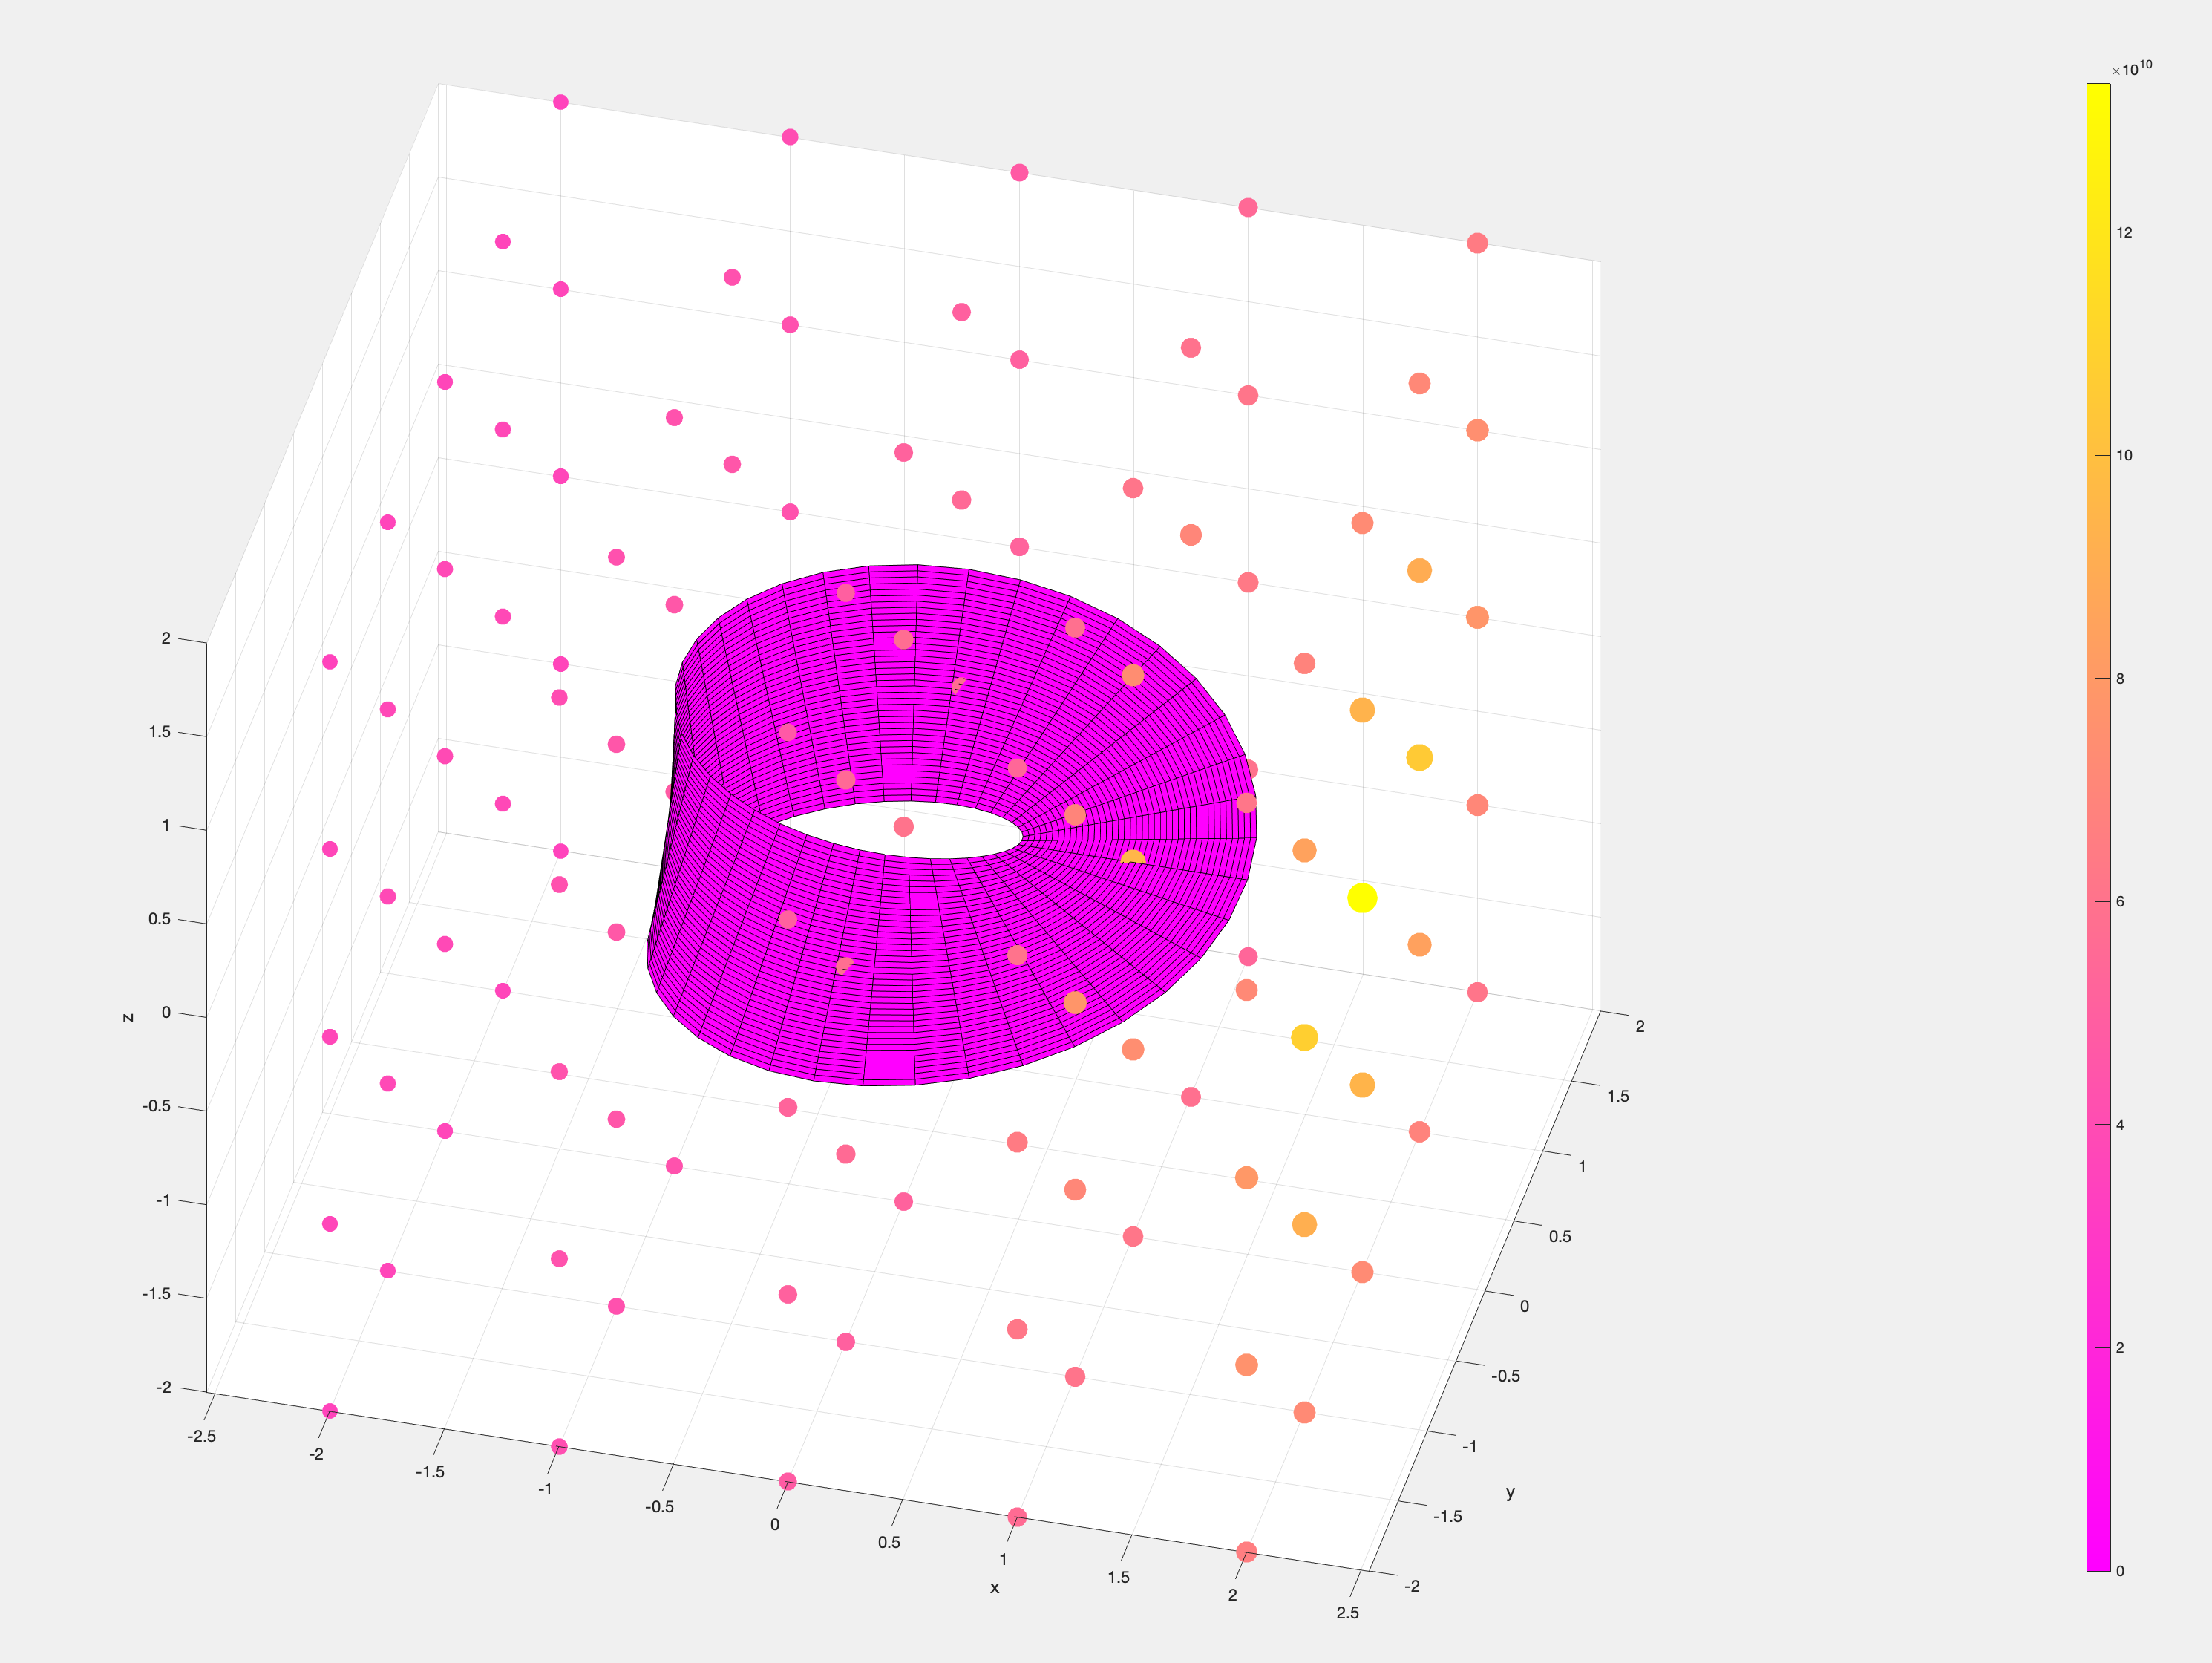
\includegraphics[width=0.7\textwidth]{U.png}
  \caption{莫比乌斯带周围电势的分布}\label{UUU}
\end{figure}

从图中可以看出,靠近莫比乌斯带面的地方,电场强度矢量基本垂直于该面切平面,与法向量平行。
此外,y坐标大的地方,电场强度更大;距中心圆点相同距离的点x坐标大的,电势更高。
\newpage
\begin{thebibliography}{4}%不使用BibTeX的方法;99意为参考文献的最大数值为99个,这个数可以自己设置
    \bibitem{ref0}百度百科. 莫比乌斯带[DB/OL]. (2022-11-21)[2022-12-11]. https://baike.baidu.com/item/莫比乌斯带/4457881
    \bibitem{ref00}百度文库. 莫比乌斯带——精选推荐[DB/OL]. [2022-12-11]. https://wenku.baidu.com/view/6823a462ae02de\\80d4d8d15abe23482fb4da02ca.html?$\_$wkts$\_$=1670857341735\&bdQuery=莫比乌斯带带电
    \bibitem{ref01}百度百科. 电场叠加原理[DB/OL]. (2022-11-21)[2022-12-11]. https://baike.baidu.com/item/电场叠加原理/846636
    \bibitem{ref1}知乎. 莫比乌斯带的参数方程是怎么来的?它又为什么没有方向呢?[EB/OL]. (2019-07-30)[2022-12-11]. https://zhuanlan.zhihu.com/p/75237170
    \bibitem{ref2}叶邦角. 电磁学[M]. 第2版. 合肥: 中国科学技术大学出版社, 2018: 28-47.
\end{thebibliography}

\backmatter
\bibliography{bib/ustc.bib}  % 参考文献使用 BibTeX 编译 
% \printbibliography       % 参考文献使用 BibLaTeX 编译

\end{document}
